\documentclass{beamer}

\usepackage{amsmath}
\usepackage{amssymb}
\usepackage{framed}

\begin{document}


\begin{frame}
%---------------------------------------------------- %
\begin{figure}
\vspace{1cm}
\centering

\includegraphics[width=0.37\linewidth]{./Rlogo}

%\label{fig:RlogoMAM}
\end{figure}
\LARGE
\[ \mbox{Shiny Demonstration}  \]

\[ \mbox{West of Ireland Data Science}  \]
\Large


\[ \mbox{26th February 2015}  \]
\end{frame}
%---------------------------------------------------- %
\begin{frame}
\begin{figure}
\Large
\centering

\includegraphics[width=0.55\linewidth]{./Rstudio}
\[ \mbox{shiny.rstudio.com}  \]
%\label{fig:RlogoMAM}
\end{figure}

\end{frame}

\begin{frame}
%--------------------------------------------------%
\frametitle{RStudio}
\LARGE
\begin{itemize}
\item Makers of Shiny : RStudio\\ (JJ Allaire, Hadley Wickham etc etc)
\item RStudio? IDE for \texttt{R}. See \texttt{www.rstudio.org} for more.
\item Shiny's  Lead Developers : Winston Chang and Joe Cheng.
\end{itemize}

\end{frame}
%---------------------------------------------------- %
\begin{frame}
\frametitle{Overview of Demonstration}
\Large
\textbf{Overview of Demonstration}
\begin{itemize}
%\item Some Announcements
\item Resources (i.e. Shiny Tutorial Page)
\item Minimal Examples 
\item Widgets
\item A bit about JavaScript
\item Special Design Considerations
\item Deploying Shiny
\end{itemize}
\end{frame}
%---------------------------------------------------- %
%---------------------------------------------%
%\begin{frame}
%\frametitle{London R - December Meeting}
%
%\begin{description}
%\item[Date:]  Tuesday 3rd December
%
%\item[Time:]  6pm (presentations begin at 6.30pm)
%
%\item[Venue:]  Balls Brothers, Minster Pavement, Mincing Lane, London EC3R 7PP
%\item[Info:] See \texttt{www.LondonR.org} for more details.
%\end{description}
%%-----------%
%\textbf{Presentations:}
%\begin{description}
%\item[Andy South] - Making beautiful world maps with country-referenced data using rworldmap and other R packages
%\item[Malcolm Sherrington] - Algorithmic Trading with R
%\item[Chris Beeley] - Shiny happy web interfaces - Shiny, HTML, CSS, JavaScript, and Shiny Server working together
%\end{description}
%\end{frame}

%---------------------------------------------%
%---------------------------------------------------- %
\begin{frame}
\Large
\frametitle{What is Shiny?}
\textbf{Easy web applications in R}\\
\textit{(Source: Shiny's Website)}
\begin{itemize}
\item \textbf{\textit{Shiny}} makes it super simple for \texttt{R} users like you to turn analyses into interactive web applications that anyone can use. \item Let your users choose input parameters using friendly controls like sliders, drop-downs, and text fields. \item Easily incorporate any number of outputs like plots, tables, and summaries.
\end{itemize}
\end{frame}
%---------------------------------------------------- %
%---------------------------------------------------- %
\begin{frame}
\Large
\frametitle{What is Shiny?}
\vspace{-1cm}
\textbf{Easy web applications in R (contd.)}\\
\textit{(Source: Shiny's Website)}
\begin{itemize}
\item No \textbf{HTML} or \textbf{JavaScript} knowledge is necessary. If you have some experience with \texttt{R}, you’re just minutes away from combining the statistical power of \texttt{R} with the simplicity of a web page.
\item \textit{(Remark: They do appear to be really handy - based on several examples  available on the internet!)}
\end{itemize}

\end{frame}
%---------------------------------------------------- %
\begin{frame}
	\begin{figure}
\centering

\includegraphics[width=0.7\linewidth]{shinytutorials}

\end{figure}

\end{frame}

%---------------------------------------------------- %
\begin{frame}
\Large
\frametitle{Shiny Resources}
\vspace{-1.5cm}
\textbf{Resources}
\begin{itemize}

\item Shiny Tutorial - (\texttt{shiny.rstudio.com/tutorial/})
\item Chris Beeley's Book\\ (Sample Chapter Available)
\item Stack-Overflow and GitHub 
\end{itemize}

\end{frame}
\begin{frame}
%---------------------------------------------------- %
\begin{figure}
\vspace{0.5cm}
\centering

\includegraphics[width=0.75\linewidth]{./snap2}

%\label{fig:RlogoMAM}
\end{figure}
\Large
\[ \mbox{Matthew Leonawicz (SNAP - Uni. Alaska Fairbanks)}  \]
\[\mbox{github.com/ua-snap/shiny-apps}‎\]
\[ \mbox{twitter.com/leonawicz} \]

\end{frame}

%---------------------------------------------------- %
\begin{frame}
\begin{figure}

\centering

\includegraphics[width=0.55\linewidth]{./github}
\[ \mbox{github - code sharing}  \]
%\label{fig:RlogoMAM}
\end{figure}
\Large


\end{frame}


%---------------------------------------------------- %
\begin{frame}
	\frametitle{Components of Shiny}
	\Large
	\textbf{Main Components of a Shiny Web App} 
	\begin{itemize}
		\item The shiny app is structurally a folder. The name of the app is the name of the folder.
		\item  Shiny programs are the easiest to build and
		understand using two scripts, which are kept within this folder. They must be
		named \texttt{server.R} and \texttt{ui.R}.
		\item 
		The input elements are defined in
		\texttt{ui.R} and processed by \texttt{server.R}, which then sends them back to \texttt{ui.R}
		\item Consideration: \textbf{\textit{Reactive Programming}}
	\end{itemize}
	
	
\end{frame}
\begin{frame}
\begin{figure}
\centering
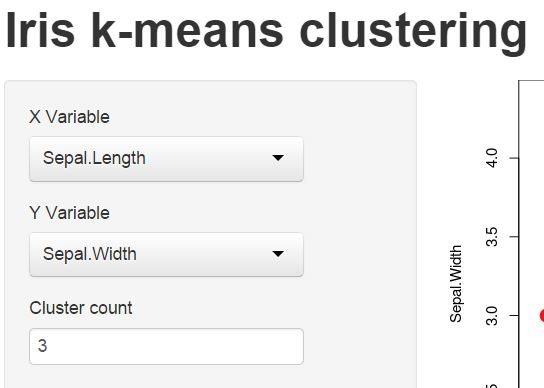
\includegraphics[width=0.9\linewidth]{00-sidebar}

\end{figure}

\end{frame}
\begin{frame}
	\begin{figure}
\centering
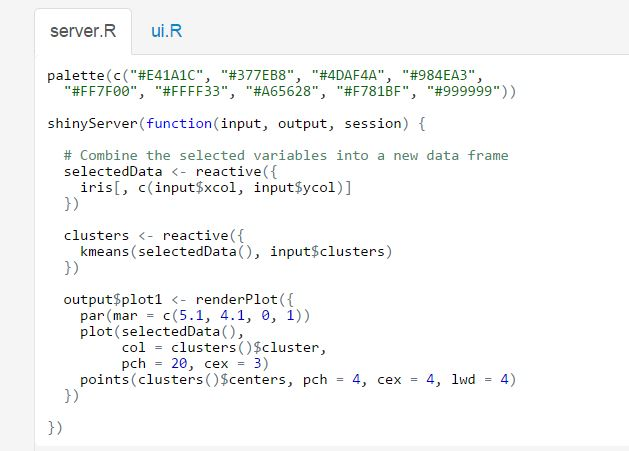
\includegraphics[width=0.9\linewidth]{00-server}

\end{figure}

\end{frame}
\begin{frame}
	\begin{figure}
\centering
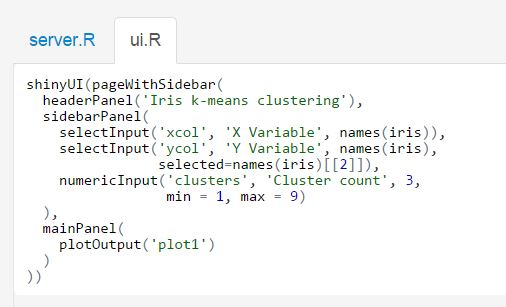
\includegraphics[width=0.9\linewidth]{00-ui}

\end{figure}

\end{frame}
\begin{frame}
	\begin{figure}
		\centering
		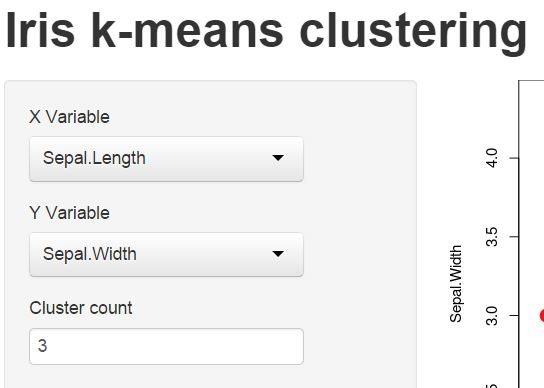
\includegraphics[width=0.9\linewidth]{00-sidebar}
		
	\end{figure}
	
\end{frame}

\begin{frame}
	\begin{figure}
\centering
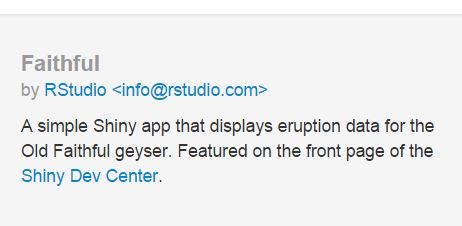
\includegraphics[width=0.\linewidth]{01-faithful}
\caption{}
\label{fig:01-faithful}
\end{figure}

\end{frame}
\begin{frame}
\begin{figure}
	\centering
	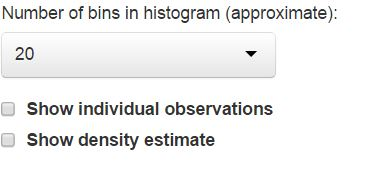
\includegraphics[width=0.9\linewidth]{01-sidebar}
\end{figure}
\end{frame}
\begin{frame}
	\begin{figure}
		\centering
		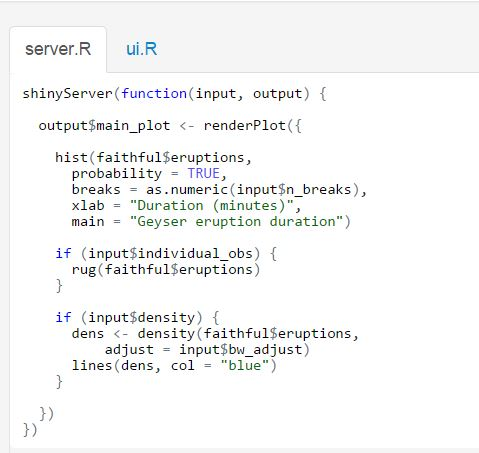
\includegraphics[width=0.9\linewidth]{01-server}
	\end{figure}
\end{frame}

\begin{frame}
	\begin{figure}
		\centering
		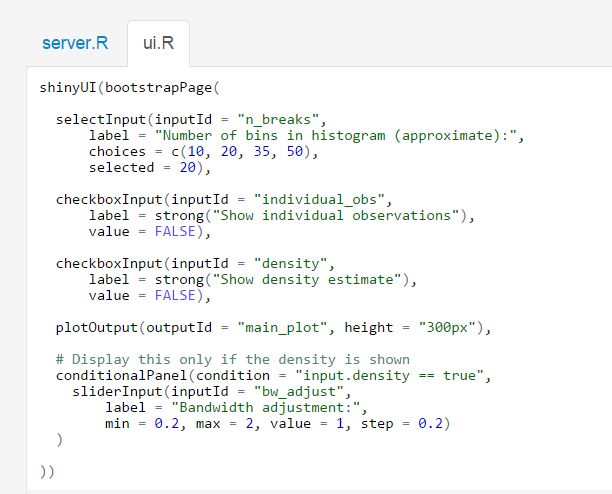
\includegraphics[width=0.9\linewidth]{01-ui}
	\end{figure}
\end{frame}

%----------------------------------------------------- %
\section{Ractive Programming}
\begin{frame}[fragile]
	\Large
	\frametitle{Reactive Programming}
	
	Simple \texttt{R} example re: reactivity
	\begin{framed}
		\begin{verbatim}
		> A <- 5
		> B <- A + 3
		> A <-6         #Update A
		>
		> c(A,B,A+3)
		[1] 6 8 9
		>
		\end{verbatim}
	\end{framed}
	Comapre this with Microsoft Excel Spreadsheets
\end{frame}

%-----------------------------------------------%
\begin{frame}
	\frametitle{Shiny Basics}
	\Large
	\vspace{-0.5cm}
	\textbf{Basic structure of a Shiny program}
	\begin{itemize}
		\item  Selection of simple input widgets (checkboxes and radio buttons)
		\item  Selection of simple output types (rendering plots and returning text)
		\item  Selection of simple layout types (page with sidebar and tabbed output panel)
		\item  Handling reactivity in Shiny
	\end{itemize}
\end{frame}

%-----------------------------------------------%
\begin{frame}[fragile]
	\frametitle{Running a Shiny App}
	\Large
	To run a Shiny program on your local machine you just need to do the following:
	\begin{enumerate}
		\item  Make sure that \texttt{server.R} and \texttt{ui.R} are in the application subfolder (\texttt{appName}).
		\item Make the main folder \texttt{R}'s working directory (using the \texttt{setwd()} command, for
		example \texttt{setwd("~/shinyFiles")}).
		\begin{verbatim}
		>...\shinyFiles\appName
		\end{verbatim}
		\item Load the Shiny package (\texttt{library(shiny})). You
		should always do that in both \texttt{server.R} and \texttt{ui.R} files.
	\end{enumerate}
	
	
\end{frame}
%-----------------------------------------------%
\begin{frame}
	\frametitle{runApp}
	\Large
	\vspace{-1.5cm}
	\begin{itemize}
		\item Type \texttt{runApp("appName")} at the console.
		%\item runApp() with the name of a directory within works just as well, for example,runApp("~/shinyFiles/minimalExample").
		\item If you are in the application folder, just type \texttt{runApp()}
		\item \textbf{Important} - Just remember that it is a directory
		and not a file that you need to point to.
	\end{itemize}
\end{frame}


%-----------------------------------------------%
\begin{frame}
	\frametitle{ui.R}
	\Large
	\textbf{User Inferface}
	\begin{itemize}
		\item The \texttt{ui.R} file is a description of the UI and is often the shortest and simplest part of
		a Shiny application. \item All of the UI elements are defined
		within this instruction.
		\item The standard shiny layout is a three panel layout, with a header panel, a sidepanel 
		controls on the left, and the main panel on the right - with the output.
		\item This layout is called \textbf{\emph{pageWithSidebar}}. There are other layouts too - such as \textbf{\textit{basicPage}} and \textbf{\textit{threePage}}.
	\end{itemize}
	
\end{frame}
%-----------------------------------------------%
\begin{frame}
	\Large
	%-----------------------------------------------%
	\frametitle{Inputs}
	The arguments are pretty typical among most of the widgets and are
	as follows:
	\begin{description}
		\item[ inputId]: This argument names the variable so it can be referred to in the
		\texttt{server.R} file
		\item[ label]: This argument gives a label to attach to the input so users know
		what it does
		\item[value]: This argument gives the initial value to the widget when it is
		set up. \\\textit{All the widgets should have sensible defaults for this argument.}
	\end{description}
\end{frame}
%-----------------------------------------------%

%-----------------------------------------------%
\begin{frame}
	\frametitle{Main Panel}
	\Large
	\vspace{-1cm}
	\begin{itemize}
		\item The final function is \texttt{mainPanel()}, which sets up the output window. 
		\item  HTML helper functions - make a little title \texttt{h3("...")}. Knowledge of HTML is very useful!
		\item There are several of these functions designed to generate HTML to go straight on
		the page; \\e.g. type \texttt{?p} at the console for the complete list. 
	\end{itemize}
\end{frame}
%-----------------------------------------------%
%-----------------------------------------------%
\begin{frame}
	\Large
	\frametitle{Main Panel}
	\begin{itemize}
		\item The other element that goes in
		\texttt{mainPanel()} is an area for handling reactive text or plots generated within the\texttt{ server.R}
		file
		\item For example - a call to \texttt{textOutput()} with the name of the output as defined in
		\texttt{server.R}, in the upcoming "minimal case" examples.
		% "textDisplay".
	\end{itemize}
\end{frame}
%=====================================================================================%
\begin{frame}[fragile]	
\frametitle{Layout of a Shiny Web Application}
\Large
\textbf{\texttt{fluidPage} - updated}
\begin{itemize}
	\item To create a display with a fluid, unbroken layout, Shiny \texttt{ui.R} scripts need the function \texttt{fluidPage}. Shiny knows where to put your app’s elements when it reads them in the \texttt{fluidPage} function.
	
	\item The following \texttt{ui.R} script creates a user-interface that has a title panel, a sidebar panel, and a main panel. 
	\item Note that these elements are placed within the \texttt{fluidPage()} function.
\end{itemize}
\end{frame}

%=====================================================================================%
\begin{frame}[fragile]	
\frametitle{Layout of a Shiny Web Application}
	\begin{framed}
		\begin{verbatim}
		# ui.R
		
		shinyUI(fluidPage(
		titlePanel("title panel"),
		
		sidebarLayout(
		sidebarPanel( "sidebar panel"),
		mainPanel("main panel")
		)
		))
		\end{verbatim}
	\end{framed}
	
\end{frame}
%=====================================================================================%
\begin{frame}[fragile]
\frametitle{Layout of a Shiny Web Application}
\begin{itemize}	
	\item \texttt{titlePanel} and \texttt{sidebarLayout} are the two most popular elements to add to \texttt{fluidPage}. They create a basic Shiny app with a sidebar.
	\begin{itemize}
	\item \texttt{sidebarLayout} always takes two arguments:
	\item \texttt{sidebarPanel} function output
	\item \texttt{mainPanel }function output
	\end{itemize}
	\item These functions place content in either the sidebar or the main panels.
	\item 
	By default the sidebar appears on the left side of your app’s display. To move the sidebar to the right, in \texttt{sidebarLayout} set position to “right.”
\end{itemize}
\end{frame}
%=====================================================================================%
\begin{frame}[fragile]
\frametitle{Layout of a Shiny Web Application}
\begin{framed}
	\begin{verbatim}
	# ui.R
	
	shinyUI(fluidPage(
	titlePanel("title panel"),
	
	sidebarLayout(position = "right",   #<- HERE
	sidebarPanel( "sidebar panel"),
	mainPanel("main panel")
	)
	))
	\end{verbatim}
\end{framed}

\end{frame}

%=====================================================================================%
\begin{frame}
	%-----------------------------------------------%
	\frametitle{server.R}
	\Large
	
	\begin{itemize}
		\item \texttt{shinyServer(...{...})} defines the bit of Shiny that's
		going to handle all the data. 
		\item On the whole, two types of things go in here. \item \textbf{Reactive
			objects} (for example, data) are defined, which are then passed around as needed (for
		example, to different output instructions), \item Outputs are defined, such as graphs.
	\end{itemize}
\end{frame}
%-----------------------------------------------%


\begin{frame}
	\frametitle{Shiny - Special Topics}
	\LARGE
	\begin{itemize}
		\item Conditional Panels - Outside Document
		\item Formatted Text - Outside Document
		
		\item HTML - Outside Document
		
		\item MathsJax
	\end{itemize}
	
	
\end{frame}

%------------------------------------- %
\begin{frame}
	\frametitle{Sliders Widgets and Tabs}
\textbf{Customizing Sliders}
\begin{itemize}
\item Shiny slider controls are extremely capable and customizable.
\item Features supported include:
	\begin{itemize}
	\item The ability to input both single values and ranges
	\item Custom formats for value display (e.g for currency)
	\item The ability to animate the slider across a range of values
	\end{itemize}
	\item Slider controls are created by calling the sliderInput function. 
%The ui.R file demonstrates using sliders with a variety of options:
\end{itemize}
\end{frame}
%------------------------------------- %
%%------------------------------------- %
%\begin{frame}
%	\frametitle{Sliders}
%	\textbf{Server Script
%	The server side of the Slider application is very straightforward: it creates a data frame containing all of the input values and then renders it as an HTML table:
%\end{frame}
%------------------------------------- %
%------------------------------------- %
\begin{frame}[fragile]
	\frametitle{Widgets}
Worked Example  - ex10
	\begin{verbatim}
	sidebarPanel(
	selectInput("dataset", "Choose a dataset:", 
	choices = c("rock", "pressure", "cars")),
	
	numericInput("obs", "Number of observations to view:", 10),
	
	helpText("Note: while the data view will show only the specified",
	"number of observations, the summary will still be based",
	"on the full dataset."),
	
	submitButton("Update View")
	)
	\end{verbatim}
\end{frame}
%------------------------------------- %
%%------------------------------------- %
%\begin{frame}
%	\frametitle{Widgets}
%	
%\end{frame}
%------------------------------------- %
%------------------------------------- %
\begin{frame}
	\frametitle{Tab Panels}
	\begin{itemize}
	\item Tabsets are created by calling the \texttt{tabsetPanel} function with a list of tabs created by the \texttt{tabPanel} function. 
	\item Each tab panel is provided a list of output elements which are rendered vertically within the tab.
	
	\item In this example we updated our Hello Shiny application to add a summary and table view of the data, each rendered on their own tab. 
\end{itemize}
%Here is the revised source code for the user-interface:
\end{frame}
%------------------------------------- %
%------------------------------------- %
\begin{frame}[fragile]
	\frametitle{Widgets}
Worked Example  - 	ex11
	\begin{framed}
		\begin{verbatim}
		mainPanel(
		tabsetPanel(
		tabPanel("Plot", plotOutput("plot")), 
		tabPanel("Summary", verbatimTextOutput("summary")), 
		tabPanel("Table", tableOutput("table"))
		)
		)
		\end{verbatim}
	\end{framed}
\end{frame}
%------------------------------------- %


%---------------------------------------------%
\begin{frame}
	\frametitle{Deploying Shiny apps}
	\Large
	\vspace{-1cm}
	\begin{itemize}
		\item  The Shiny package itself is designed to run Shiny applications locally. 
		\item To share Shiny applications with other R users, you can send them your application source as a GitHub gist, R package, or zip file.
	\end{itemize}
\end{frame}

\begin{frame}
	\frametitle{Deploying Shiny}
	\Large
	\textbf{Sharing Apps to Run Locally}
	\begin{itemize}
		\item Once you’ve written your Shiny app, you can distribute it for others to run on their own computers—they can download and run Shiny apps with a single \texttt{R} command. All that this requires that they have \texttt{R} and Shiny installed on their computers.
		
		\item If you want your Shiny app to be accessible over the web, so that users only need a web browser, see Deploying Shiny Apps over the Web.
	\end{itemize}
	%Here are some ways to deliver Shiny apps to run locally:
	
\end{frame}
%-----------------------------------------------------------------------------------%
\begin{frame}
	\frametitle{Deploying Shiny}
	\Large
	\textbf{Gist}
	\begin{itemize}
		\item One easy way is to put your code on gist.github.com, a code pasteboard service from \textbf{GitHub}. 
		\item Both \texttt{server.R} and \texttt{ui.R} must be included in the same gist, and you must use their proper filenames. 
		\item See \textit{http://gist.github.com/3239667} for an example.
	\end{itemize}
\end{frame}
%-------------------------------------------------------------------------%
\begin{frame}[fragile]
	\Large
	\begin{itemize}
		\item Your recipient must have R and the Shiny package installed, and then running the app is as easy as entering the following command:
		
		\begin{framed}
			\begin{verbatim}
			shiny::runGist('3239667')
			\end{verbatim}
		\end{framed}
		\item In place of '\textit{\textbf{3239667}}' you will use your gist’s ID; or, you can use the entire URL of the gist (e.g. '\textit{https://gist.github.com/3239667}').
	\end{itemize}
\end{frame}

\begin{frame}
	\Large
	\frametitle{Deploying Shiny}
	\textbf{Advantages of using Gist} 
	\begin{itemize}
		\item Source code is easily visible by recipient (if desired)
		\item Easy to run (for \texttt{R} users)
		\item Easy to post and update
	\end{itemize} 
	\textbf{Cons} \begin{itemize}
		\item Code is published to a third-party server
	\end{itemize}
\end{frame}

%-----------------------------------------------------------------------------------%
\begin{frame}[fragile]
	\Large
	\textbf{GitHub repository}
	\begin{itemize}
		\item If your project is stored in a git repository on GitHub, then others can download and run your app directly. An example repository is at \textit{\textbf{http://github.com/rstudio}}
		\item The following command will download and run the application:
	\end{itemize}
	\large
	\begin{framed}
		\begin{verbatim}
		shiny::runGitHub(`shiny_example', `rstudio')
		\end{verbatim}
	\end{framed}
	\normalsize
	\textit{In this example, the GitHub account is 'rstudio' and the repository is 'shiny example'; you will need to replace them with your account and repository name.}
\end{frame}

\begin{frame}
	\Large
	\textbf{Github: Advantages} \begin{itemize}
		\item  Source code is easily visible by recipient (if desired)
		\item Easy to run (for R users)
		\item Very easy to update if you already use GitHub for your project
		\item Git-savvy users can clone and fork your repository
	\end{itemize} \textbf{Disadvantages} \begin{itemize}
	\item Developer must know how to use git and GitHub.
	\item Code is hosted by a third-party server.
\end{itemize}
\end{frame}


%-----------------------------------------------------------------------------------%
\begin{frame}[fragile]
	\frametitle{Deploying Shiny}
	\textbf{Making it into a Package}
	\begin{itemize}
		\item If your Shiny app is useful to a broader audience, it might be worth the effort to turn it into an \texttt{R} package. Put your Shiny application directory under the package’s inst directory, then create and export a function that contains something like this:
		\begin{framed}
			\begin{verbatim}
			shiny::runApp(system.file('appdir', 
			package='packagename'))
			\end{verbatim}
		\end{framed}
		where \texttt{appdir} is the name of your app’s subdirectory in inst, and \textbf{\emph{packagename}} is the name of your package.
	\end{itemize}
\end{frame}

\begin{frame}
	\frametitle{Deploying Shiny}
	\textbf{Making it into a Package}:\\ \bigskip
	\textbf{Advantages} \begin{itemize}
		\item Publishable on CRAN
		\item Easy to run (for \texttt{R} users)
	\end{itemize} \textbf{Disadvantages} \begin{itemize}
	\item More work to set up
	\item Source code is visible by recipient (if not desired)
\end{itemize}
\end{frame}

%---------------------------------------------%
\begin{frame}
	\frametitle{Deploying Shiny apps}
	\Large
	\textbf{Deployment over the Web}
	\begin{itemize}
		\item You can also deploy Shiny applications over the web, so that users need only a web browser and your application’s URL.
		\item For this, you’ll need a Linux server and our Shiny Server software. 
		\item Shiny Server is free and open source, though in the future RStudio will offer a commercially licensed edition with additional features for larger organizations.
		\item RStudio also working on a subscription-based hosting service for Shiny. 
	\end{itemize}
\end{frame}
%---------------------------------------------%

\begin{frame}
	\frametitle{Deploying Shiny apps : Shiny Server}
	\Large
	\textbf{Shiny Server}
	\begin{itemize}
		
		
		\item Shiny Server is if you want to use your own server instead of hosting it on Rstudio's server (i.e. \textbf{\textit{glimmer}}). 
		
		\item  This is really important for those who can't let their code or data out of their organization, 
		or want more computational/storage resources than glimmer can offer, or need their apps to access their 
		internal network.
	\end{itemize}
\end{frame}
%---------------------------------------------%

\end{document}
%---------------------------------------------------- %
